
\begin{frame}{Updating Parameters}
\begin{itemize}
    \item Computation of gradients is similar as standard MLP.
    \item Keep in mind the parameters of RNNs are shared through time steps. 
    \item Sometime backprop for RNNs is called backprop through time (BPTT). 
    \item No need to go through its details as DL frameworks compute gradients. 
    \item If you would like to compute gradients brute-force, you can do that numerically. 
    \begin{itemize}
        \item for each weight $w$, compute $\frac{\text{Loss}(w+h) - \text{Loss}(w)}{h}$, 
        \item weight update after gradient computation is as in SGD $w \longleftarrow w - \alpha \frac{\partial \text{Loss}}{\partial w}$
    \end{itemize}
\end{itemize}
\end{frame}

\begin{frame}{Updating Parameters}
\begin{itemize}
    \item RNNs can be seen as a very very deep neural model with sparse and skip connections
    \item The output of last steps are calculated based on the hidden state vectors at early steps
    \item Recall 1:
    \begin{equation*}
    \begin{split}
            \bm{z^{(h)}_t} & = \bm{x_t}U + \bm{h_{t-1}}W + \bm{b_h} \\
            \bm{h_t} & =  f \big( \bm{z^{(h)}_t} \big) \\
    \end{split}
    \end{equation*}
    \item Recall 2:
        \begin{equation*}
        \begin{split}
            \bm{z^{(\hat{y})}_t} & = \bm{h_t}V + \bm{b_{\hat{y}}}  \\ 
            \bm{\hat{y}_t} & =  g \big(  \bm{z^{(\hat{y})}_t} \big) 
            \end{split}
        \end{equation*}

\end{itemize}    
\end{frame}

\begin{frame}{Updating Parameters}
\centering
\begin{itemize}
    \item Recall 1:
        \begin{equation*} \bm{z^{(h)}_t}  = \bm{x_t}U + \bm{h_{t-1}}W + \bm{b_h}
        \end{equation*}
        \begin{equation*}
        \bm{h_t}  =  f\big( \bm{z^{(h)}_t} \big)
        \end{equation*}
    \item Recall 2:
            \begin{equation*}
            \bm{z^{(\hat{y})}_t} = \bm{h_t}V + \bm{b_{\hat{y}}}  
            \end{equation*}
            \begin{equation*}
            \bm{\hat{y}_t}  =  g\big(  \bm{z^{(\hat{y})}_t} \big) 
        \end{equation*}
    \item If we have only two steps: 
    \begin{equation*}
        \frac{\partial \text{Loss}}{ \partial \bm{W}} 
         = \sum_{t=1}^{2}   \frac{\partial \ell_t}{\partial \bm{W}} = \frac{\partial \ell_1}{\partial \bm{W}}  + \frac{\partial \ell_2}{\partial \bm{W}}  
    \end{equation*}
    \begin{equation*}
        \frac{\partial \ell_1}{\partial \bm{W}}  = 
        \frac{\partial \ell_1}{\partial \bm{\hat{y_1}}} \frac{\partial \bm{\hat{y_1}}}{\partial \bm{z^{(\hat{y})}_1}}  
        \frac{\partial \bm{z^{(\hat{y})}_1}}{\partial  \bm{h_1}}  
        \frac{\partial \bm{h_1}}{\partial \bm{z^{(h)}_1}}
        \frac{\partial \bm{z^{(h)}_1}}{\partial \bm{W}}  \propto   \textcolor{myblue}{\frac{\partial \bm{h_1}}{\partial \bm{z^{(h)}_1}}}
    \end{equation*}
    \begin{equation*}
    \frac{\partial \ell_2}{\partial \bm{W}}  = 
    \frac{\partial \ell_2}{\partial \bm{\hat{y_2}}} \frac{\partial \bm{\hat{y_2}}}{\partial \bm{z^{(\hat{y})}_2}}  
    \frac{\partial \bm{z^{(\hat{y})}_2}}{\partial  \bm{h_2}}  
    \frac{\partial \bm{h_2}}{\partial \bm{z^{(h)}_2}}\bm{h_1}\frac{\partial \bm{h_1}}{\partial \bm{z^{(h)}_1}}
        \frac{\partial \bm{z^{(h)}_1}}{\partial \bm{W}} \propto  
        \textcolor{myblue}{
        \frac{\partial \bm{h_2}}{\partial \bm{z^{(h)}_2}}\frac{\partial \bm{h_1}}{\partial \bm{z^{(h)}_1}}
        }
    \end{equation*}
     
\end{itemize}    
\end{frame}

\begin{frame}{Updating Parameters}
\centering
\begin{itemize}
    \item If we have  three steps: 
    \begin{equation*}
        \frac{\partial \text{Loss}}{ \partial \bm{W}} 
         = \sum_{t=1}^{3}   \frac{\partial \ell_t}{\partial \bm{W}} = \frac{\partial \ell_1}{\partial \bm{W}}  + \frac{\partial \ell_2}{\partial \bm{W}} + \frac{\partial \ell_3}{\partial \bm{W}}
    \end{equation*}
    \begin{equation*}
        \frac{\partial \ell_1}{\partial \bm{W}}  \propto   \textcolor{myblue}{\frac{\partial \bm{h_1}}{\partial \bm{z^{(h)}_1}}}
    \end{equation*}
    \begin{equation*}
    \frac{\partial \ell_2}{\partial \bm{W}}  \propto  
        \textcolor{myblue}{
        \frac{\partial \bm{h_2}}{\partial \bm{z^{(h)}_2}}\frac{\partial \bm{h_1}}{\partial \bm{z^{(h)}_1}}
        }
    \end{equation*}
    \begin{equation*}
    \frac{\partial \ell_3}{\partial \bm{W}}  \propto  
        \textcolor{myblue}{
        \frac{\partial \bm{h_3}}{\partial \bm{z^{(h)}_3}}\frac{\partial \bm{h_2}}{\partial \bm{z^{(h)}_2}}\frac{\partial \bm{h_1}}{\partial \bm{z^{(h)}_1}}
        }
    \end{equation*}     
\end{itemize}    
\end{frame}

\begin{frame}{Updating Parameters}
\centering
\begin{itemize}
    \item If we have  $n$ steps: 
    \begin{equation*}
        \frac{\partial \text{Loss}}{ \partial \bm{W}} 
         = \sum_{t=1}^{3}   \frac{\partial \ell_t}{\partial \bm{W}} = \frac{\partial \ell_1}{\partial \bm{W}}  + \frac{\partial \ell_2}{\partial \bm{W}} + \frac{\partial \ell_3}{\partial \bm{W}}
    \end{equation*}
    \begin{equation*}
        \frac{\partial \ell_1}{\partial \bm{W}}  \propto   \textcolor{myblue}{\frac{\partial \bm{h_1}}{\partial \bm{z^{(h)}_1}}}
    \end{equation*}
    \begin{equation*}
    \frac{\partial \ell_2}{\partial \bm{W}}  \propto  
        \textcolor{myblue}{
        \frac{\partial \bm{h_2}}{\partial \bm{z^{(h)}_2}}\frac{\partial \bm{h_1}}{\partial \bm{z^{(h)}_1}}
        }
    \end{equation*}
    \begin{equation*}
    \frac{\partial \ell_3}{\partial \bm{W}}  \propto  
        \textcolor{myblue}{
        \frac{\partial \bm{h_3}}{\partial \bm{z^{(h)}_3}}\frac{\partial \bm{h_2}}{\partial \bm{z^{(h)}_2}}\frac{\partial \bm{h_1}}{\partial \bm{z^{(h)}_1}}
        }
    \end{equation*}
    \begin{equation*}
        ...
    \end{equation*}
        \begin{equation*}
    \frac{\partial \ell_n}{\partial \bm{W}}  \propto  
        \textcolor{myblue}{
        \frac{\partial \bm{h_n}}{\partial \bm{z^{(h)}_n}} ...\frac{\partial \bm{h_3}}{\partial \bm{z^{(h)}_3}}\frac{\partial \bm{h_2}}{\partial \bm{z^{(h)}_2}}\frac{\partial \bm{h_1}}{\partial \bm{z^{(h)}_1}}
        }
    \end{equation*}     
\end{itemize}    
\end{frame}
\begin{frame}{Exploding Gradients}
    \begin{itemize}
        \item Given: 
                \begin{equation*}
    \frac{\partial \ell_n}{\partial \bm{W}}  \propto  
        \textcolor{myblue}{
        \frac{\partial \bm{h_n}}{\partial \bm{z^{(h)}_n}} ...\frac{\partial \bm{h_3}}{\partial \bm{z^{(h)}_3}}\frac{\partial \bm{h_2}}{\partial \bm{z^{(h)}_2}}\frac{\partial \bm{h_1}}{\partial \bm{z^{(h)}_1}}
        }
    \end{equation*}     
        if all the gradients in the chain are greater than one then their multiplications explodes
        \begin{equation*}
            \frac{\partial \ell_n}{\partial \bm{W}} = \text{NaN}
        \end{equation*}
    \end{itemize}
\end{frame}
\begin{frame}{Vanishing Gradients}
    \begin{itemize}
        \item Given: 
                \begin{equation*}
    \frac{\partial \ell_n}{\partial \bm{W}}  \propto  
        \textcolor{myblue}{
        \frac{\partial \bm{h_n}}{\partial \bm{z^{(h)}_n}} ...\frac{\partial \bm{h_3}}{\partial \bm{z^{(h)}_3}}\frac{\partial \bm{h_2}}{\partial \bm{z^{(h)}_2}}\frac{\partial \bm{h_1}}{\partial \bm{z^{(h)}_1}}
        }
    \end{equation*}     
        if one of the gradients in the chain is close to zero or all gradients are less than one then their multiplications vanishes
        \begin{equation*}
            \frac{\partial \ell_n}{\partial \bm{W}} = 0.0
        \end{equation*}
    \end{itemize}
\end{frame}

\begin{frame}{Vanishing and Exploding Gradients}
    \begin{itemize}
        \item Why are such gradients a problem? 
        \item  In case of exploding gradients,  the learning is very unstable
        \item The last steps become independent from the early steps 
        \item The prediction at each step is conditioned only on a few previous steps 
        \item These problems also happen in MLPs with many hidden layer where we use the Sigmoid activation function

    \end{itemize}
\end{frame}

\begin{frame}{Vanishing and Exploding Gradients}
    
Some sings that show a model and its training may suffer from these problems:
        \begin{itemize}
            \item a very high loss on training set or no learning
            \item large changes in loss on each update due to the models instability
            \item loss becomes NaN during training
            \item model weights grow exponentially during training (explosion)
            \item the model does not learn during training
            \item training stops very early and any further training does not decrease the loss
            \item the weights closer to the last steps would  change more than those at early steps
            \item weights shrink exponentially and become very small \item the model weights become 0 in the training phase.
        \end{itemize}
\end{frame}
\begin{frame}{Simple Remedies for Vanishing/Exploding Gradients}
    \begin{itemize}
        \item For activation of hidden layers use \texttt{ReLU}, and initialize $W$ with the identity matrix(Le et al., 2015)
        \item Gradient clipping (Pascanu et al., 2013)
        \begin{figure}
            \centering
            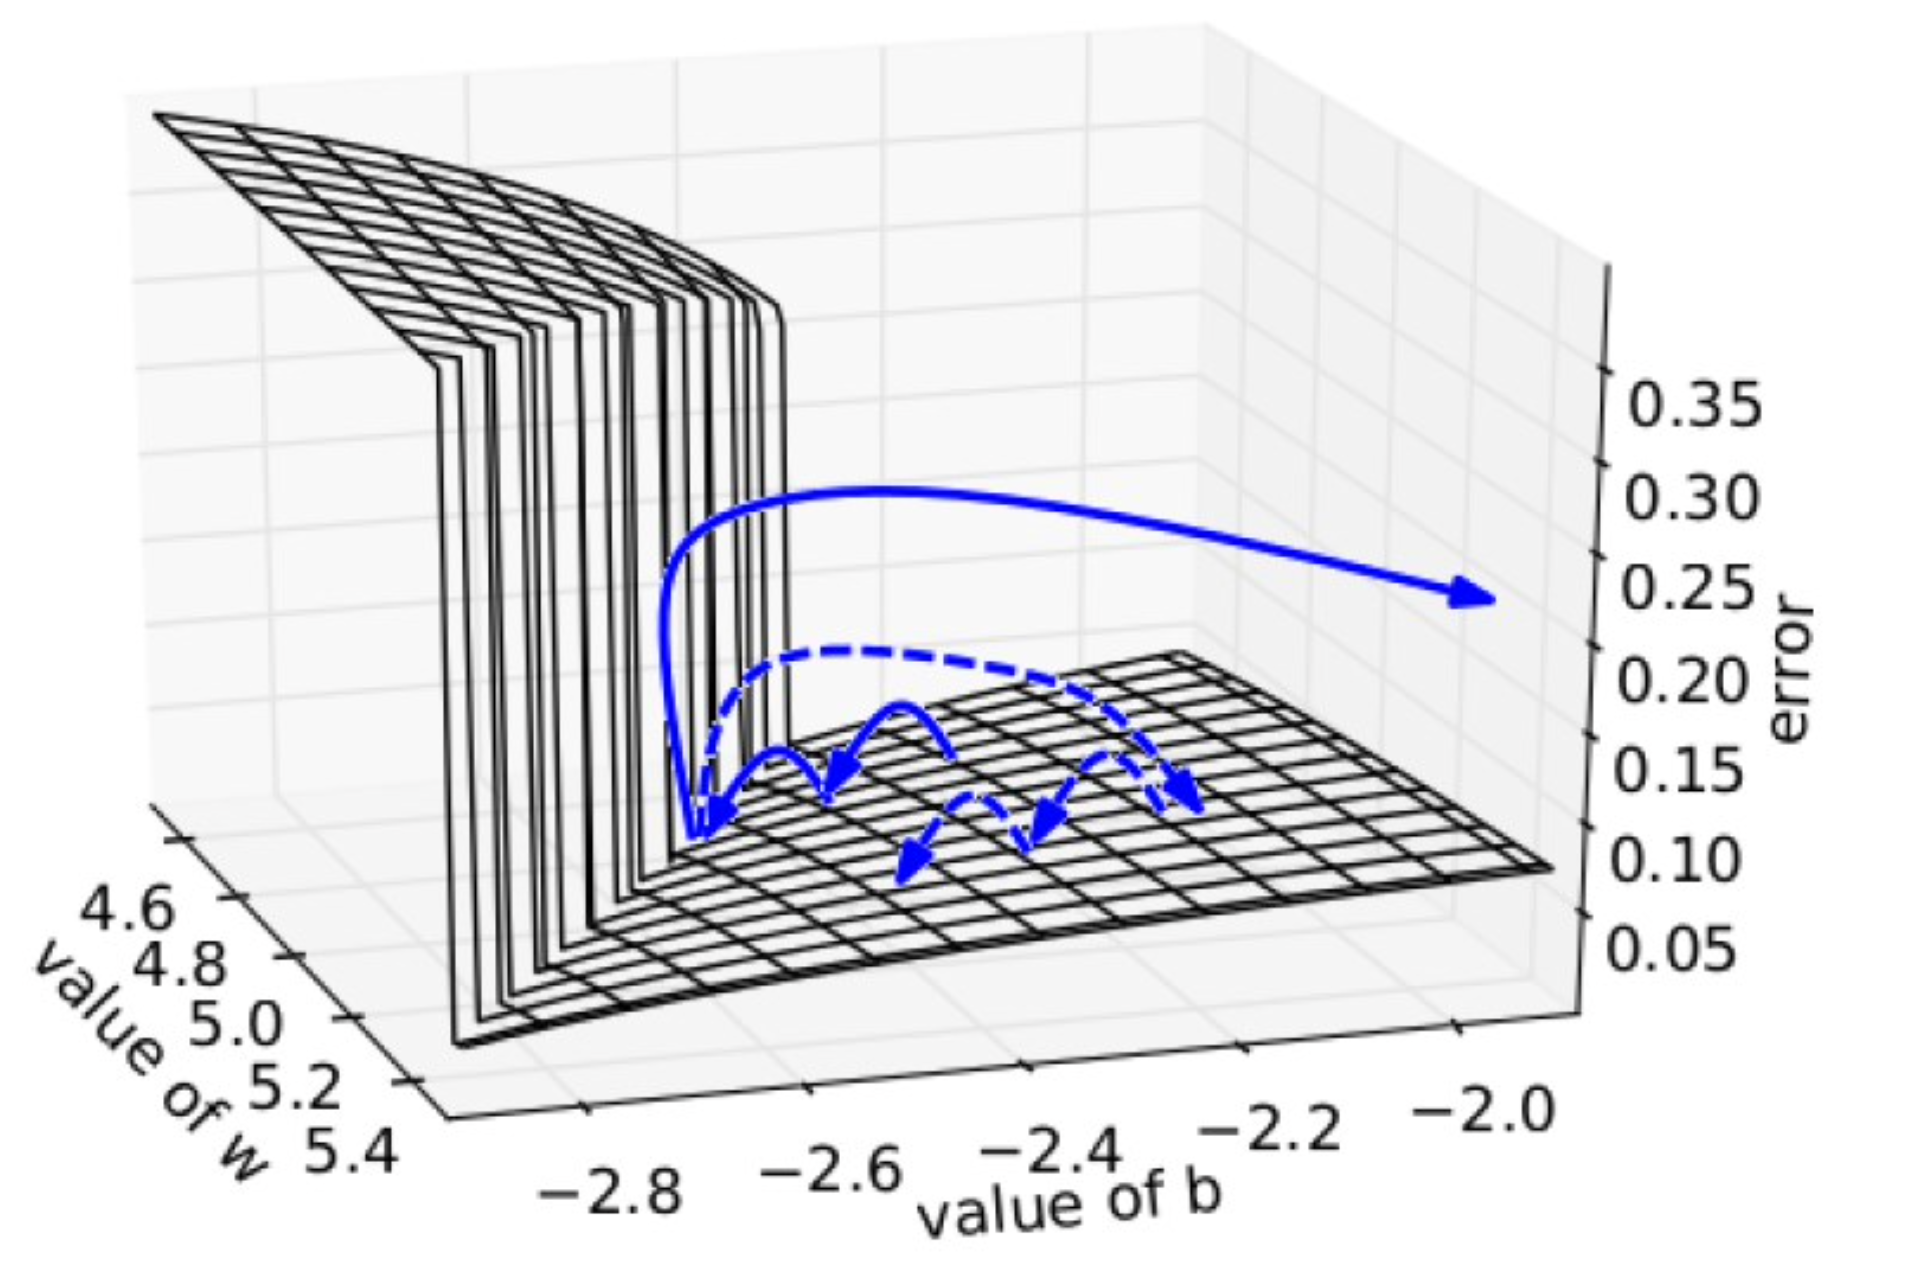
\includegraphics[scale=0.09]{./figure/gradient_clipping.png}
        \end{figure}
        \item GRUs and LSTMs
    \end{itemize}
\end{frame}
\begin{frame}{Gated Recurrent Units (GRUs)}
    \begin{itemize}
        \item GRUs are introduced by Cho et al., (2014)
        \item more advanced method for hidden state representation
        \item The key idea behind GRUs is to enable hidden states to capture long distance dependencies
    \end{itemize}
\end{frame}
